% !TEX root = ../main.tex

\section*{1}

Let denote LB and UB as a lower bound and upper bound of
of maximum number that an arbitrary line can intersect with a
triangulation $T$ of $n$. We claim that :

\begin{align*}
    \mathrm{LB} &= 2\\
    \mathrm{UB} &= \text{No. Triangles in T} + 1
\end{align*}
\begin{figure}[h]
    \begin{center}
        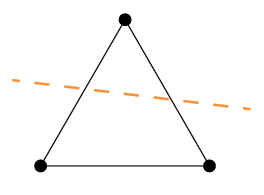
\includegraphics[width=0.5\textwidth]{smallest-triangulation}
        \caption{Smallest Triangulation}
        \label{fig:smallest-triangulation}
    \end{center}
\end{figure}

To prove LB, it is obvious to see from Figure \ref{fig:smallest-triangulation}
the smallest triangulation, that the maximum number of intersection is $2$.
